
\documentclass{../templates/llncs}
\usepackage{../templates/salt-light}
\usepackage{makeidx}
\usepackage{url}
\usepackage{graphicx}
\usepackage{array}

\begin{document}

\title{Cooking HTTP content negotiation with Vapour} % FIXME

\author{Diego Berrueta\inst{1}, Sergio Fern\'andez\inst{1} and Iv\'an Frade\inst{2}}

\institute{
Fundaci\'on CTIC\\
Gij\'on, Asturias, Spain\\
\email{\{diego.berrueta,sergio.fernandez\}@fundacionctic.org\\http://www.fundacionctic.org/}
\and
Universidad de Oviedo\\
Oviedo, Asturias, Spain\\
\email{ivan.frade@gmail.com\\http://www.uniovi.es/}
}

\maketitle

\begin{abstract}
The Semantic Web is built upon distributed knowledge published on 
the Web. But this vision cannot be implemented without some basic publishing
rules to make the data readable for machines. Publication of RDF vocabularies
must receive special attention due to their important role 
in the Semantic Web architecture. In this paper we describe a scripting 
web-based application that validates the compliance of a vocabulary 
against these publication rules. Practical experimentation allows to 
illustrate and to discuss some common problems in the implementation
of these rules.
\end{abstract}

\section{Introduction}

The Semantic Web is a big container, a universal medium for data, information
and knowledge exchange. However the Semantic Web is not only about putting data on
the Web, there are some publishing rules. Tim Berners-Lee outlined four basic 
principles~\cite{TimBL2006} to publish Linked Data on the Web~\cite{PublishLinkedData2007}.
These rules describe how \texttt{URIs} must be used as names for things, 
and how to provide useful information on these things and other related 
ones. Although there are guidelines to coin adequate URIs for 
things~\cite{Sauermann2007}, there is still the need to provide the best 
representation of the information for each request depending on each kind 
of client agent, human or software.

Web documents are retrieved using mainly the HTTP~\cite{HTTP} 
protocol. This protocol provides a mechanism known as \textit{content negotiation}. 
By means of content negotiation, it is possible to serve Web content in the format or 
language preferred by the requester (if it is available, obviously). Using transparent content negotiation 
in HTTP~\cite{Holtman1998} has many benefits~\cite{Seshan1998}, and it can be implemented
using different techniques in the Apache web server, as we describe in more detail in 
Section~\ref{sec:contentnegotiation} of this paper. Section~\ref{sec:vapour} introduces 
a scripting application that provides help and guidance to implement correctly and to debug
HTTP content negotiation. In Section~\ref{sec:experimental} the
compliance of some of the most used
vocabularies in the Semantic Web is evaluated with respect to the publishing rules. Finally, Section~\ref{sec:conclusions} presents 
some conclusions and future work.


\section{\label{sec:contentnegotiation}Content negotiation with Apache: Recipes}

%FIXME: something generic about content negotiation
%an image explaining content negotiation?
%something like http://www.w3.org/TR/cooluris/img20071212/303.png

Nowadays, the Apache HTTP Server is the most used Web server\footnote{\url{http://www.netcraft.com/survey/} (retrieved 13/Mar/2008)}, 
and it provides three different approaches to implement content negotiation\footnote{\url{http://httpd.apache.org/docs/2.0/content-negotiation.html}}:

\begin{description}

  \item \textbf{Type Map:} Explicit handlers are described in a file (.var) for 
        each resource. The necessary configuration is quite complicated and 
        tedious, therefore this method is hardly used.

  \item \textbf{MultiViews:} Based in the MIME-type and names of the files 
        in a directory, MultiViews serves the most appropriate file in the current 
        directory when the requested resource does not exist. It returns 
        an additional header (\texttt{Content-Location}) to indicate the actual 
        location of the file. This method can be extended using the Apache module \texttt{mod\_mime} 
        to associate handlers to new file extensions. However, this solution
        has a quite important problem: it only works if the files exist in
        the same directory.

  \item \textbf{Rewrite request:} Probably because the two alternatives above
        do not provide an easy solution, the most widely used method is one 
        which was not specifically designed to implement content negotiation. 
        This mechanism uses the module \texttt{mod\_rewrite} in order to rewrite the 
        request according to some ad-hoc rules.
        As a result, requests (for objects that are not known to be information resources)
        are redirected using the HTTP 303 status code, to the URI of the appropriate
        content depending on the format requested.
        Obviously,  
        some time is lost with the extra HTTP round-trip, but it is negligible for
        many applications,
        as well as mandatory according the httpRange-14 resolution from the
        TAG\footnote{\url{http://www.w3.org/2001/tag/issues.html#httpRange-14}}.

\end{description}

There is some ongoing work by W3C on \textit{Best Practice Recipes for Publishing 
RDF Vocabularies}~\cite{Recipes}, a document which contains several recipes that advice on how 
to publish RDF/OWL Vocabularies using \texttt{mod\_rewrite}. This ``cookbook'' 
provides step-by-step instructions to publish vocabularies on the Web, and gives
example configurations designed to address the most common scenarios.

However, the \textit{Recipes} are not perfect, and there is at least one important issue to 
be solved\footnote{\url{http://www.w3.org/2006/07/SWD/track/issues/58} (retrieved 13/Mar/2008)}.
Tim Berners-Lee reported that ``the recipe for responding to an accept 
header only responds to a header which EXACTLY matches [the rule antecedent]''.
For those requests which contain values for the Accept header such as 
\texttt{text/*} or \texttt{application/rdf+xml;q=0.01}, where wildcards or
$q$-values are used, the actual representation served by the
rules proposed in the \textit{Recipes} might differ from the expected one. This is a serius problem
of the \textit{Recipes}, but it can be easily solved using a script at server-side.

%Probably it might be solved by moving to another 
%technique, or with a combination of these commented techniques.

%FIXME: solution ISSUE #58 !!!
%http://lists.w3.org/Archives/Public/public-swd-wg/2007Jul/0177.html

\section{\label{sec:vapour}Vapour: a scripting approach to debug content negotiation}
%FIXME: find a better title for this section

The previous section has shown that a correct implementation of content negotiation 
is not an easy task. Futhermore, manually testing an implementation is not complex, but
it is long and cumbersome. Although it can be done with tools such as 
cURL\footnote{Richard Cyganiak's explanation of how to use cURL to debug content negotiation, 
blog post available at: \url{http://dowhatimean.net/2007/02/debugging-semantic-web-sites-with-curl}}, this process is not handy, specially for intensive or repetitive tests against a vocabulary.

\begin{figure}
 \centering
 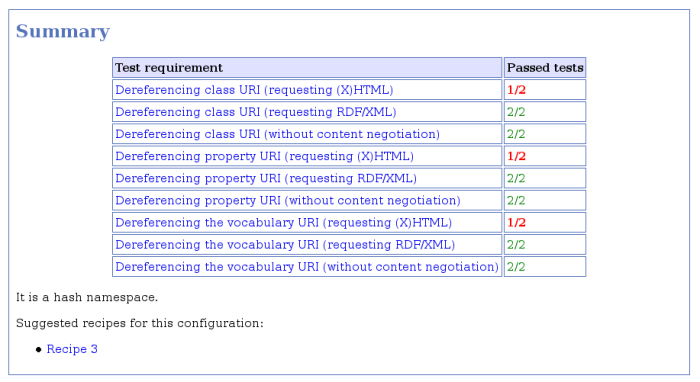
\includegraphics[width=12cm]{images/report-summary.png}
 \caption{\label{fig:report-summary}Example of a report summary made by Vapour.}
\end{figure}

In order to facilitate the task of testing the results of content 
negotiation on a vocabulary, we developed a web-based application 
called Vapour\footnote{\url{http://vapour.sourceforge.net/}}. This 
application provides a service that makes multiple requests to a set 
of URIs and runs a test suite specifically designed to check the responses 
of the server against the best practices defined in the \textit{Recipes}.
Tests are executed against the vocabulary
URI, a class URI and a property URI (the latter two can be automatically detected).
Based on the input parameters, the application provides a pointer to the specific
recipe, in case the user wants to learn more on how to configure the web server. 
Vapour stores all assertions into an in-memory RDF store, using a combination of EARL~\cite{EARL}, HTTP
Vocabulary~\cite{Koch2007} and an RDF representation of the best practices of the \textit{Recipes}. 
Thus Vapour can provide the reports both in HTML and in RDF, using content
negotiation. The HTML view displays a clean and concise pass/fail report of each 
set of tests (Figure~\ref{fig:report-summary}), as  well as a detailed explanation 
of its findings that includes a graphical representation of the HTTP dialog. Needless 
to say, the examples included in the \textit{Recipes} are successfully validated by 
Vapour.

The application is written in Python, and it uses common
Python libraries such as urllib, httplib, web.py and RDFLib. Scripting languages such 
as Python allow an agile development of applications in a short time with little 
resources. Source code of Vapour is available on 
SourceForge\footnote{\url{http://sourceforge.net/projects/vapour/}},
and an online demo of the service is also available\footnote{\url{http://idi.fundacionctic.org/vapour}}.

\begin{figure}
 \centering
 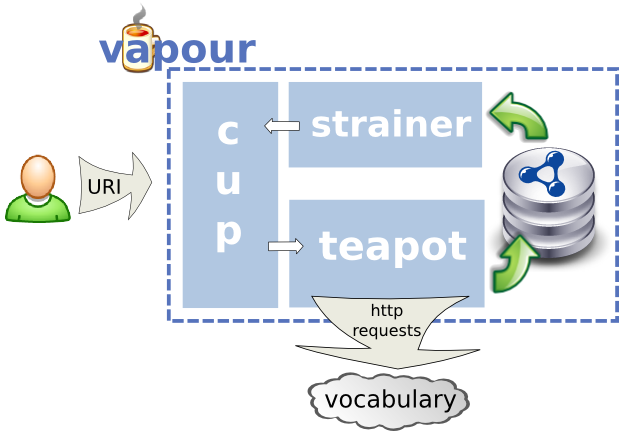
\includegraphics[width=8cm]{images/arch.png}
 \caption{\label{fig:arch}High level architecture of Vapour.}
\end{figure}

As depicted in Figure~\ref{fig:arch}, Vapour has a simple and functional
design that fulfils the objectives of the project. There are three components:

\begin{description}

  \item \textbf{cup} is the web front-end. It uses the web.py framework
        and the Cheetah template engine, and it provides a web interface that allows 
        the user to interact with other components of the application in a 
        simple way. The architecture has been designed to allow other kind 
        of interfaces. For instance, a command line interface is also provided.

  \item \textbf{teapot} is the core of the application. It launches
        HTTP dialogs 
        (with and without content negotiation) to evaluate the response
        status code and content-type. Teapot requests the URI of the vocabulary, and 
        also the URIs of a class and a property from the vocabulary. All the resulting assertions are 
        inserted into the RDF store.

  \item \textbf{strainer} is the module in charge of generating the reports for
        each test performed by the application. It queries the RDF model using SPARQL %~\cite{SPARQL} 
        to get the result and trace of each test, and it produces 
        a report in XHTML or RDF/XML. For the XHTML reports, we also use Cheetah 
        templates.

\end{description}

The service can be deployed as a normal CGI in Apache or using a Python web 
framework. We reviewed the security of the application avoiding some common 
problems in this kind of applications, such as limiting requests per client.

\section{\label{sec:experimental}Experimental results}

Practical experimentation illustrates some common problems of how
content negotiation is implemented, and enables the discussion on 
these problems. We checked some RDFS and OWL vocabularies published on the web.
We chose the most frequently used vocabularies, in terms of number of
instances, according to the last scientific study~\cite{Li2005}. However,
this ranking is aging (2004), so we also included some newer
vocabularies, such as SKOS, DOAP and SIOC, which are also popular
according to more up-to-date sources\footnote{See the ranking at http://pingthesemanticweb.com/stats/namespaces.php (retrieved 12/Mar/2008) by PingTheSemanticWeb.com~\cite{Bojars2007}}.

\begin{table}[t]
\caption{Ratio of passed tests / total tests for a list of widely used vocabularies in the semantic web.}
\centering
\begin{tabular}{lccc}
\hline
Namespace & Accept & Accept & Default \\
 & RDF & HTML & response \\
\hline\hline
\texttt{http://www.w3.org/1999/02/22-rdf-syntax-ns\#} & 3/3 & N/A & RDF/XML \\
\texttt{http://www.w3.org/2000/01/rdf-schema\#} & 3/3 & N/A & RDF/XML \\
\texttt{http://xmlns.com/foaf/0.1/} & 3/3 & 3/3 & HTML \\
\texttt{http://purl.org/dc/elements/1.1/} & 2/2 & 0/2 & RDF/XML \\
\texttt{http://www.w3.org/2003/01/geo/wgs84\_pos\#} & 3/3 & 0/3 & RDF/XML \\
\texttt{http://rdfs.org/sioc/ns\#} & 3/3 & 0/3 & RDF/XML \\
\texttt{http://www.w3.org/2004/02/skos/core\#} & 3/3 & 3/3 & RDF/XML \\
\texttt{http://usefulinc.com/ns/doap\#} & 3/3 & 0/3 & RDF/XML \\
\texttt{http://purl.org/rss/1.0/} & 1/3 & 0/3 & HTML \\
\texttt{http://semantic-mediawiki.org/swivt/1.0\#} & 0/3 & 0/3 & text/plain \\ [1ex]
\hline
\end{tabular}
\label{tab:usage}
\end{table}

Table~\ref{tab:usage} summarizes the results of running Vapour against a list of
ten popular vocabularies of the semantic web. These results provide an
approximation to the quality of the publication of vocabularies on the web. 
All the vocabularies were retrieved on 12/Mar/2008. For each vocabulary, the vocabulary URI, a class URI and a property URI were tested
(except for Dublin Core, which does not have any class). The results show that
most vocabularies are correctly published as RDF. However, it is significant that
most vocabularies do not correctly provide HTML representations of the resources, even
if they are available.
Additionally, some vocabularies return an incorrect MIME type,
such as \texttt{text/plain} or \texttt{application/xml}.

\section{\label{sec:conclusions}Conclusions}

Content negotiation is a powerful technique. Although the basic mechanism is simple,
it is often badly implemented. Vapour is useful to debug and to provide advice on how to solve common problems, as well as to provide quality 
assurance in the best possible way.

%FIXME: delete this (off topic) paragraph???
%As we have seen, it is still necessary to solve as soon as possible some 
%important issues in the actual document of the Recipes. While we do not 
%find the most correct way to do it, maybe a \textit{push} action from the Web 
%community will be necessary to develop a new module that allows to serve 
%Linked Data in the correct way with content negotiation.

The application presented in this paper is fairly simple, but  
it actually helps to debug the implementation of content negotiation in web servers. It
is particularly interesting that Vapour provides the results also in RDF . Using this machine-readable 
format, it should be easy to build another service on top of Vapour, and to use these data for 
other tasks, such as a service to check the compliance of a specific collection 
of vocabularies published on the Web.

Current best practices (and consequently, Vapour) should probably be
updated to cover new methods to publish RDF data, such as
RDFa~\cite{Birbeck2006} embedded in XHTML pages. In the future, we would like
to extend Vapour to cover more generic validations in Linked
Open Data scenarios, and to help webmasters to better understand some common
implementation issues.

% ---- Bibliography ----
\bibliographystyle{abbrv}
\bibliography{../references}

\end{document}
